\ifdefined\chinchin
	\documentclass[12pt, orivec]{extarticle} % 12pt, 14pt, 17pt, 20pt
\else
	\documentclass[10pt, orivec]{extarticle} % 12pt, 14pt, 17pt, 20pt
\fi
\usepackage{parskip}
\usepackage{amsmath}
\usepackage{amssymb}    % for \rightsquigarrow
\usepackage{wasysym}	% for frown face
\usepackage{mathrsfs} 	% for \mathscr
\usepackage{stmaryrd}
% \usepackage{unicode-math}
\usepackage[many]{tcolorbox}
\usepackage{ulem}
\usepackage{tikz-cd}		% commutative diagrams
\usepackage{tikz}
\usepackage{amsthm}
\usepackage{enumitem}	% for \ietemize custom labels
\usepackage{turnstile}	% longer turnstiles
\usepackage[sf,bf,big,raggedright,compact]{titlesec}	% change section color to blue
\usepackage{graphicx}	% Allows including images
% \usepackage[backend=biber,bibstyle=authoryear,citestyle=../authoryearbrack]{biblatex}
% \bibliography{../AGI-book}

\newtheorem{theorem}{Theorem}

\ifdefined\chinchin
	\newcommand{\cc}[2]{#1}
	\usepackage[CJKspace]{xeCJK}
	%\setCJKmainfont[BoldFont=SimHei,ItalicFont=AR PL KaitiM GB]{Alibaba PuHuiTi}
	\setCJKmainfont[Path={/usr/share/fonts/truetype/Alibaba PuHuiTi/}, BoldFont=Alibaba_PuHuiTi_Regular.ttf, ItalicFont=ukai.ttc]{Alibaba_PuHuiTi_Light.ttf}
	% \setmainfont[ItalicFont=Latin Modern Roman Slanted]{Alibaba Sans:style=Light}
\else
	\newcommand{\cc}[2]{#2}
	% \usepackage[no-math]{fontspec}
	% \setmainfont[Path={/usr/share/fonts/opentype/Alibaba Sans/},
	% BoldFont=Alibaba_Sans_Regular.otf,
	% ItalicFont=Alibaba_Sans_Light_Italic.otf]
	% {Alibaba_Sans_Light.otf}
	%\setmainfont{AlibabaSans_Light.otf}
	%\renewcommand{\baselinestretch}{0.8}
\fi

%\setlength{\headheight}{0cm}
%\setlength{\hoffset}{0cm}
%\setlength{\topmargin}{-2cm}
%\setlength{\oddsidemargin}{-2cm}
%\setlength{\evensidemargin}{-2cm}
%\setlength{\textwidth}{20cm}
%\setlength{\textheight}{26cm}
%\setlength{\headsep}{0.5em}
%\setlength{\topskip}{0.5em}
%\setlength{\footskip}{0.9cm}  % between bottom of page and page number
%\setlength{\floatsep}{0cm}
%\setlength{\textfloatsep}{0.6cm}
%\setlength{\intextsep}{0.5cm}
%\setlength{\parindent}{0em}   % em = width of capital M
%\setlength{\parskip}{10pt plus 5pt}

% Fix spilling of titles in bibliography:
%\DeclareFieldFormat*{title}{#1}
%
%\DeclareFieldFormat*{titlecase}{%
%    \ifdef{\currentfield}
%      {\ifcurrentfield{title}
%         {\usefield{\uline}{\currentfield}}%
%         {#1}}
%      {#1}}

\setcounter{secnumdepth}{1}		% 0 = no section numbers

\titleformat{\section}[hang]{\bfseries\Large\color{blue}}{\thesection \hspace{20pt}}{0pt}{}
\titleformat{\subsection}[hang]{\bfseries\large\color{blue}}{\thesubsection \hspace{10pt}}{0pt}{}
\titleformat{\subsubsection}[hang]{\bfseries\color{blue}}{}{0pt}{}

\itemsep1em
% \setlist[itemize]{noitemsep, topsep=15pt, partopsep=10pt}
\setlist[itemize]{topsep=15pt, partopsep=10pt}
\renewcommand{\labelitemi}{\textbullet}

\let\varzero\emptyset
\let\emptyset\varnothing		% round empty set
\newcommand{\vect}[1]{\symbf{#1}}
\newcommand{\book}[1]{$\NewSym[0.4]{../book-icon.png} \quad$ \parbox{0.9\textwidth}{\footnotesize #1}}
\newcommand{\code}[1]{{\small{\ttfamily #1}}}
\newcommand{\tab}{\hspace*{2cm}}
\newcommand{\powerset}{\raisebox{.15\baselineskip}{\Large\ensuremath{\wp}}}
\newcommand{\Chi}{\raisebox{2.5pt}{$\chi$}}
\newcommand*\KB{\vcenter{\hbox{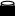
\includegraphics{../KB-symbol.png}}}}
\newcommand*\NewSym[2][0.5]{\vcenter{\hbox{\includegraphics[scale=#1]{#2}}}}
\newcommand*\sigmoid{\vcenter{\hbox{
\includegraphics{../sigmoid3.png}}}}
\newcommand{\smbox}[1]{\boxed{\footnotesize{\mbox{#1}}}}

\newcommand{\tikzmark}[1]{\tikz[overlay,remember picture] \node (#1) {};}

\newcommand{\Dfrac}[2]{%
\ooalign{%
      $\genfrac{}{}{2.9pt}0{\hphantom{#1}}{\hphantom{#2}}$\cr%
      $\color{white}\genfrac{}{}{1.5pt}0{\hphantom{#1}}{\hphantom{#2}}$\cr%
      $\color{white}\genfrac{}{}{1pt}0{\color{black}#1}{\color{black}#2}$}}

% \renewcommand{\thefootnote}{\fnsymbol{footnote}}
%\usepackage{perpage}
%\MakePerPage{footnote}
%\renewcommand{\thefootnote}{\ifcase\value{footnote}\or{*}
%	\or{$\dagger$}\or{**}\or{$\ddagger$}\fi}
%\renewcommand{\thefootnote}{\arabic{footnote}}
%\setcounter{footnote}{0}

\usepackage[hang,flushmargin]{footmisc}
\interfootnotelinepenalty=10000
